\chapter{Environment per Sistemi Esperti}
Il numero di ambienti di sviluppo per sistemi esperti è cresciuto negli anni e con esso il numero e la tipologia di funzionalità offerte. Le prime \emph{shell} erano semplici metodi di rappresentazione della conoscenza basata sull'uso delle regole, con il supporto di strumenti di inferenza piuttosto limitati. Con gli anni, la lista e la tipologia di funzionalità offerte si è arricchita introducendo una varietà di possibilità per la rappresentazione della conoscenza, strategie di ricerca, meccanismi specializzati di inferenza e strumenti di supporto allo sviluppo dei sistemi.

L'evoluzione di questi sistemi è stata motivata con il tempo e la quantità di sforzo richiesto per la costruzione di sistemi esperti usando linguaggi tradizionali e sistemi strettamente vincolati all'uso della regole per la rappresentazione della conoscenza.

L'obiettivo inseguito con l'evoluzione degli ambienti di sviluppo era quello di ridurre i tempi ed i costi di sviluppo dei sistemi esperti. Inoltre l'uso di questi strumenti ha garantito:
\begin{itemize}
	\item un miglioramento generale della qualità e l'affidabilità dei sistemi prodotti
	\item di astrarre l'attività di sviluppo del sistema esperto da quelle relative allo sviluppo dell'ambiente di base
	\item agli ingegneri della conoscenza la possibilità di focalizzarsi sugli aspetti correlati alla modellazione degli elementi del dominio del sistema esperto
	\item di utilizzare strumenti rapidi per l'acquisizione e la modifica della conoscenza dei sistemi esperti
\end{itemize}

I miglioramenti hanno incrementato in questo modo le possibilità di successo nello sviluppo di sistemi esperti. Come ulteriore effetto, il ridursi della complessità generale delle operazioni realizzazione ha consentito di gestire e produrre soluzioni di sempre maggiore complessità.

\section{Evoluzione degli strumenti di sviluppo}
Tornando indietro agli albori della produzione di sistemi esperti, i meccanismi di inferenza e le basi di conoscenza erano strettamente accoppiati fra loro. La prima generazione di sistemi non era altro che grandi applicazioni scritte in linguaggi come LISP. Nonostante tutti i linguaggi di programmazione possano essere utilizzati per la produzione di sistemi esperti, alcuni di essi offrivano caratteristiche che rendevano la stessa attività più agevole. Esempi di linguaggi largamente utilizzati per queste attività sono il linguaggio LISP e Prolog. Purtroppo, la quantità di tempo e sforzo richiesto per la produzione usando queste tipologie di linguaggi diventava rapidamente insostenibile con l'aumentare della complessità. Inoltre, l'accoppiamento fra funzionalità necessarie all'inferenza e quelle per la rappresentazione e la gestione della conoscenza non permetteva una distinzione di ruoli fra gli ingegneri di sistema e quelli della conoscenza.

\subsection{Expert System Shell}

Questo approccio alla lavorazione venne superato nella successiva generazione. Durante la creazione di sistemi esperti di seconda generazione come MYCIN, i ricercatori si accorsero dell'importanza di implementare i sistemi in modo che fosse possibile una separazione, più o meno netta, fra la base di conoscenza e i meccanismi per la sua rappresentazione dalle funzionalità atte all'implementazione del motore inferenziale e i meccanismi dello stesso.

Rimuovendo la conoscenza di dominio da questi sistemi vennero realizzati i primi sistemi di tipo \emph{Skeletal Shell} o \emph{Expert System Shell} utilizzando gli strumenti sviluppati nel progetto originale e inserendo nuova conoscenza di dominio era possibile creare una grande verità di nuovi sistemi esperti con un sforzo relativamente ridotto. I sistemi di seconda generazione di maggior successo hanno dato vita a \emph{Shell} per lo sviluppo di sistemi esperti. Sono esempi EMYCIN, KAS e EXPERT: rispettivamente questi ultimi vennero prodotti rimuovendo le conoscenze di dominio da MYCIN, PROSPECTOR e CASNET.

Sebbene l'utilizzo di questi strumenti velocizzasse la produzione di nuovi sistemi di diversi ordini di magnitudine, la necessità di attenersi alle strategie utilizzate nei sistemi originali rappresentava un limite alla flessibilità del sistema. Spesso le \emph{Shell} fornivano strumenti integrati e strutture che rendevano lo sviluppo dei sistemi molto più semplice ed immediato, ma limitavano le classi di problemi a cui potevano essere applicati e riducevano grandemente le scelte di design possibili per il realizzatore di sistemi esperti. \cite{development1993}

\subsection{Expert System Environment}

Il successivo passo negli strumenti di sviluppo per sistemi esperti è quello costituito dalla produzione delle prima serie di \emph{Environment per Sistemi Esperti}. L'idea alla base di questa generazione di tool era quella di realizzare delle \emph{Shell} che offrissero sistemi multipli per la rappresentazione della conoscenza, l'inferenza e il controllo insieme ad un completo ambiente di sviluppo \cite{development1993}, senza però limitare le scelte di design dei realizzatori.

Questi strumenti vennero ulteriormente arricchiti con l'integrazione di funzionalità orientate allo sviluppo come meccanismi di tracciamento delle regole e strutture per il debugging dei sistemi. Esempi di \emph{Environment} creati sono OPS5, OPS83, CLIPS, JESS.

L'utilizzo di questi sistemi si poneva come punto d'incontro fra le due generazioni precedenti: come mostrato in \figurename~\ref{fig:classificazione-tools}, nonostante l'utilizzo degli \emph{Environment} facilitasse lo sviluppo dei sistemi esperti, non riduceva la flessibilità e le opzioni di design a disposizione dello sviluppatore come per gli strumenti di seconda generazione. Spesso lo sviluppo di questi sistemi richiedeva ancora un certo grado di esperienza nell'uso di linguaggi di programmazione e conoscenze sintattiche in quanto gli ambienti ereditavano sintassi e strutture già a disposizione nei linguaggi di prima generazione (la famiglia di environment OPS ereditava una sintassi simile a quella usata in LISP \cite{brownston1985}).

\begin{figure}
\centering
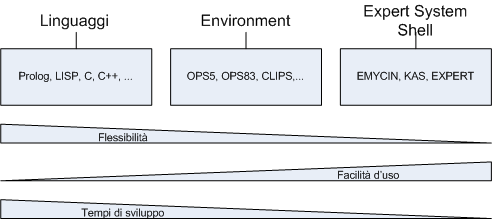
\includegraphics[scale=0.7]{Immagini/Capitolo1/classificazione-strumenti.png}
\caption{Classificazione dei tool di sviluppo per sistemi esperti}\label{fig:classificazione-tools}
\end{figure}

\section{Rappresentazione della conoscenza}
Con il termine \emph{Rappresentazione della conoscenza} ci si riferisce alle modalità con le quali la conoscenza è strutturata ed organizzata in un sistema. Fra le modalità di rappresentazione più note supportate dai tool di sviluppo per sistemi esperti sono annoverabili \emph{Regole}, \emph{Reti semantiche}, \emph{Frame} e \emph{Oggetti}. Ognuna di queste tecniche presenta vantaggi e svantaggi: alcune permettono una estrema facilità di modifica e comprensione dei sistemi, mentre altre consentono un'alta efficienza d'uso della memoria. Un ideale environment per sistemi esperti dovrebbe provvedere a supportare il maggior numero possibile di queste tecniche di rappresentazione della conoscenza \cite{development1993}, per offrire una più ampia possibilità di scelta agli sviluppatori durante le fasi di design dei sistemi.

\subsection{Regole}
La più nota forma di rappresentazione della conoscenza è quella basata su regole. \'E probabilmente un assioma dell'intelligenza artificiale, e della moderna psicologia, che comportamenti ritenuti intelligenti siano governati da regole. Anche nel mondo, le persone tendono ad associare intelligenza con coerenza nei comportamenti, e spesso il concetto di comportamento viene spiegato facendo riferimento a quello di regolarità. \cite{jackson1999}

Le \emph{regole di produzione} sono un formalismo utilizzato, in origine, nello studio delle macchine astratte, delle grammatiche formali e nella progettazione dei linguaggi di programmazione. Successivamente il loro utilizzo è approdato nell'ambito dei sistemi esperti e dell'intelligenza artificiale. Nella letteratura tecnica sono anche identificate come \emph{Regole condizione-azione} o \emph{Regole situazione-azione}. Questa nomenclatura risulta appropriata in quanto le regole sono spesso utilizzate per rappresentare, in forma codificata, associazioni fra \emph{Pattern}\footnote{Con il termine \emph{Pattern} si fa riferimento schemi di caratteristiche richieste un insieme di elementi} di dati presenti nel sistema e sequenze di azioni che il sistema stesso dovrebbe eseguire come conseguenza di un riscontro. Conseguentemente la funzione delle regole è precisamente quella di specificare regole di comportamento: forniti insiemi di dati (astraendo dalla particolare interpretazione), determinano i risultati da concretizzare.

Le produzioni sono realmente regole per la manipolazione di stringhe di simboli, chiamate spesso regole di riscrittura. Post ha studiato le proprietà dei sistemi a regole basati su produzioni, che lui stesso ha chiamato \emph{Sistemi Canonici}. Questi ultimi sono definiti come un tipo di sistemi formali basato su:

\begin{itemize}
	\item un \emph{alfabeto} A per la creazione di stringhe
	\item un insieme di stringhe considerati come \emph{assiomi}
	\item un insieme di produzioni nella forma: 
	\[
	\alpha_1\$_1 \cdots \alpha_m\$_m \rightarrow \beta_1\$_1^{'} \cdots \beta_n\$_n^{'}
	\]	
	dove
	\begin{itemize}
		\item ogni elemento $\alpha_i$ e $\beta_1$ rappresenta una stringa
		\item gli elementi $\alpha_1$ e $\alpha_m$ sono spesso nulli
		\item alcuni o addirittura tutti gli elementi $\alpha_i$ o $\beta_1$ possono essere nulli
		\item ogni $\$_i$ rappresenta una stringa variabile (che può essere la stringa nulla)
		\item ogni elemento $\$_i$ è sostituito da uno $\$_i^{'}$.
	\end{itemize}
\end{itemize}

Nell'ambito specifico dei sistemi esperti, le regole normalmente determinano come le strutture simboliche che rappresentano lo stato corrente del sistema debbano essere manipolate per avvicinare la rappresentazione stessa dello stato ad una soluzione. L'attivazione progressiva delle regole produce una \emph{catena di inferenza}.

Il concetto di regole utilizzato  all'interno dei sistemi esperti differisce da quello generico di produzioni come regole di riscrittura sotto aspetti superficiali, ma mantengono gli stessi principi fondamentali e le stesse proprietà formali.

Se da una parte nelle produzioni come regole di riscrittura l'interesse è focalizzato sulla grammatica della struttura dei simboli \emph{per se}, nell'uso delle regole come mezzi di rappresentazione della conoscenza nei sistemi esperti l'interesse è concentrato sul processo di trasformazione di una istanza del problema originale in un forma che ne rappresenti una soluzione.

Conseguentemente l'alfabeto dei \emph{sistemi canonici} è rimpiazzato da un vocabolario di simboli o atomi e da una grammatica relativamente semplice per la generazione di strutture simboliche. Normalmente il vocabolario consiste di tre insiemi:

\begin{itemize}
	\item un insieme $N$ di nomi di oggetti del dominio
	\item un insieme $P$ di nomi di proprietà che specificano attributi di un oggetto
	\item un insieme $V$ di valori che questi attributi possono assumere.
\end{itemize}

Generalmente la grammatica utilizzata prevede la specifica di triple \emph{oggetto-attributo-valore}, ma questo assunto non lede la possibilità di specifiche più espressive.

Una volta descritto un vocabolario di simboli e una grammatica per la generazione di strutture simboliche, è possibile generare una codifica della descrizione di uno stato iniziale di un problema di interesse. Questa descrizione, costituita da strutture simboliche, corrisponderà esattamente agli assiomi previsti nella definizione di \emph{sistema canonico}. La descrizione originale del problema verrà progressivamente riscritta tramite una serie di applicazioni.

Un sistema a produzioni consiste di un \emph{rules-set} (spesso anche definito come \emph{memoria delle produzioni}), un \emph{rules-interpreter} che verifica l'applicabilità delle regole e una memoria di lavoro. Il ruolo di quest'ultima componente è quella di memorizzare la descrizione iniziale del sistema, così come la descrizione finale attesa e gli stati intermedi prodotti durante la fase di elaborazione. La possibilità di attivazione delle regole è governata dall'interprete, il quale confronta la descrizione intermedia del sistema con l'insieme di regole e decide quale applicare. L'applicazione stessa delle regole (in un processo analogo a quello descritto per la riscrittura simbolica) modifica ulteriormente la descrizione del sistema presente nella \emph{working memory}.

Schematicamente questo processo può essere descritto nella forma generale
\[
C_1, \cdots, C_n \rightarrow A_1, \cdots, A_n
\]
interpretabile come:
\begin{quote}
	{\bfseries [if]} le condizioni $C_1$ e $\cdots$ e $C_n$ sono vere,\\
	{\bfseries [then]} esegui le azioni $A_1$ e $\cdots$ e $A_n$.
\end{quote}

Con i termini \emph{left-hand side} e \emph{right-hand side} si è soliti indicare rispettivamente la porzione di condizione e quella di azione di una regola.

\subsection{Reti semantiche}
Un'altra tecnica di rappresentazione della conoscenza usa reti di strutture chiamate appunto \emph{reti semantiche}. I nodi di queste reti sono costituiti da eventi, oggetti o concetti, che possono essere relazionati fra loro, tramite l'uso di archi di varia natura, per stabilire strutture gerarchie fra i concetti stessi. \cite{development1993}

Due relazioni molto comuni in questo tipo di rappresentazione sono quelle di tipo \emph{is-a} e \emph{has-part}. L'utilizzo di questa forma di rappresentazione permette una memorizzazione efficiente delle proprietà dei concetti in quanto, data la natura gerarchica implicitamente indotta dalle relazioni di ereditarietà, i nodi posti al più basso livello della rete eviteranno la ridefinizione di proprietà già deducibili dai concetti ai quali questi ultimi sono relazionati.

La definizione offerta da \emph{R. H. Richens}, ideatore delle \emph{reti semantiche}, spiega le stesse come
\begin{quote}
''una \emph{interlingua} nella quale tutte le peculiarità strutturali del linguaggio di base sono rimosse e siamo lasciati con solo quello che io chiamo una \emph{rete semantica} di \emph{idee spoglie}. In questa rete gli elementi rappresentano cose, qualità o relazioni $\cdots$[ o] punti di collegamento fra cose verso le proprie qualità o relazioni, o da qualità e relazioni verso un'ulteriore qualificazione''\cite{richens1956}
\end{quote}

\subsection{Frame}

\subsection{Oggetti}

\section{Meccanismi di inferenza}

\subsection{Controllo basato su regole}

\paragraph{Forward chaining}

\paragraph{Backward chaining}

\subsection{RETE: matching fra regole e stato}

\section{Lo scenario attuale}

\subsection{CLIPS}

\subsection{Integrazione}

\section{Obiettivi}